% ============================================================================
%  EEE3095S CS Project 2026: Serial Game Server
%  STUDENT REPORT TEMPLATE (IEEE conference format, max 10 pages incl. refs)
% ============================================================================
%
%  How to use this template
%  ------------------------
%  * Red text in [square brackets] is PLACEHOLDER text. Replace every piece of
%    it with your own words. Search the PDF for "[" before you submit.
%  * Grey boxes are GUIDANCE. They tell you what the marker looks for. Leave
%    them on while you write, then switch them off below (\guidancefalse) to
%    check your length against the 10-page limit and before you submit.
%  * Dashed boxes are PLACEHOLDER FIGURES. Replace each with your own diagram
%    (\includegraphics{figures/yourfile.pdf} or TikZ).
%  * Keep the section headings exactly as they are: they are the brief's
%    required headings, in the brief's order, and the marking guide follows
%    them. Add your own subsection headings underneath.
%  * Build:  latexmk -pdf main.tex   (or upload the folder to Overleaf).
% ============================================================================
\documentclass[conference]{IEEEtran}

\usepackage[T1]{fontenc}
\usepackage{cite}
\usepackage{amsmath}
\usepackage{graphicx}
\usepackage{booktabs}
\usepackage{array}
\usepackage{xcolor}
\usepackage{listings}
\usepackage{tikz}
\usepackage[most]{tcolorbox}
\usepackage[hidelinks]{hyperref}

% ---------------------------------------------------------------- switches --
\newif\ifguidance
\guidancefalse       % guidance boxes hidden: page count below is the real length

% ------------------------------------------------------- template helpers --
\definecolor{phred}{rgb}{0.75,0.08,0.08}
\definecolor{guidebg}{gray}{0.94}
\definecolor{guideframe}{gray}{0.55}

% Placeholder text: replace with your own.
\newcommand{\ph}[1]{\textcolor{phred}{[#1]}}

% Guidance box: what the marker expects. Hidden when \guidancefalse.
\newtcolorbox{guidebox}[1][]{
  breakable, enhanced, colback=guidebg, colframe=guideframe,
  boxrule=0.4pt, arc=1pt, left=3pt, right=3pt, top=2pt, bottom=2pt,
  fontupper=\footnotesize\sffamily, title={#1},
  fonttitle=\footnotesize\sffamily\bfseries, coltitle=black,
  colbacktitle=guidebg!80!gray, before skip=4pt, after skip=6pt}
\newenvironment{guidance}[1][Guidance]
  {\ifguidance\begin{guidebox}[#1]\else\setbox0\vbox\bgroup\fi}
  {\ifguidance\end{guidebox}\else\egroup\fi}

% Placeholder figure: dashed box with a description of what to draw.
% Usage: \figph{<height>}{<what the figure must show>}
\newcommand{\figph}[2]{%
  \begin{tikzpicture}
    \draw[dashed, phred, line width=0.6pt] (0.3pt,0) rectangle (\linewidth-0.3pt,#1);
    \node[text width=0.85\linewidth, align=center, text=phred, font=\footnotesize]
      at (0.5\linewidth,0.5*#1) {#2};
  \end{tikzpicture}}

% Protocol text in running text and tables (underscores, colons, asterisks print literally).
\newcommand{\code}[1]{\texttt{\detokenize{#1}}}
\usepackage{seqsplit}
\newcommand{\tn}[1]{\texttt{\expandafter\seqsplit\expandafter{\detokenize{#1}}}}
\newcolumntype{L}[1]{>{\raggedright\arraybackslash}p{#1}}

\lstset{
  basicstyle=\ttfamily\scriptsize, columns=fullflexible, keepspaces=true,
  frame=tb, framerule=0.4pt, commentstyle=\color{gray}\itshape,
  keywordstyle=\bfseries, showstringspaces=false, breaklines=true,
  captionpos=b, float=t, floatplacement=t,
}
\renewcommand{\lstlistingname}{Listing}

\begin{document}

% ---------------------------------------------------------------- title ----
\title{An Authoritative STM32 Tic-Tac-Toe Server with a\\
Checksummed Serial Protocol}

\author{
\IEEEauthorblockN{Hazel Kunyavapa (KNYCHI008)\quad Oswika Mukoma (MKMOSW001)}
\IEEEauthorblockA{EEE3095S CS Project 2026, Department of Electrical Engineering\\
University of Cape Town}
}

\maketitle

\begin{abstract}
We built a Tic-Tac-Toe game in which an STM32F051 is the only referee and a Python
Tkinter program is an untrusted display. The board holds the whole game in 10 bytes and
changes it only after every check of a request has passed, so a rejected request cannot
alter the game. Messages are ASCII lines of at most 32 bytes with an XOR checksum; the
server answers each frame with exactly one reply (when the client waits for it), rejects oversize, corrupt, unknown and
stalled frames with specific \code{NACK} codes, and recovers on the next valid frame. We test
the same suite of 113 pytest cases against a PC mock, against the real C logic compiled for
the PC, and against the board: all 113 pass on the board. Fifteen deliberately
injected faults are all caught by the suite, and an exhaustive PC run of the rules checks
50.5 million cases, including 6.86 million illegal moves that left the game unchanged.
\end{abstract}



\section{Introduction}
\label{sec:intro}

In a networked game, whoever holds the rules can cheat if the other side is trusted. The
brief~\cite{brief} therefore puts the referee on an STM32F051 microcontroller and treats the PC
program as an untrusted display. Our design guarantees one property: \emph{a rejected request
never changes the game}. The STM32 owns the board, the turn and the win test, and the PC only
sends requests and draws what the board confirms.

We chose Tic-Tac-Toe because its 8 winning lines and 9 cells can be checked exhaustively, which
lets us spend the effort on the protocol and the tests, as the mark scheme rewards. The PC client uses
Python's Tkinter~\cite{guilib}: it ships with Python, so a marker can run it without installing a
toolkit, and its \code{after()} polling suits our worker-thread design (Sec.~\ref{sec:design}).

Four decisions shape the system. (i)~The rules are portable C with no hardware calls, so the same
source runs on the Cortex-M0 and on a PC. (ii)~Messages are short ASCII lines with an XOR checksum, and
every frame gets exactly one reply (for clients that wait for replies). (iii)~An optional \code{NEW:AI} command makes the server play O with a minimax opponent, again through the same validated move path. (iv)~One pytest suite of 113 tests runs unchanged against a
Python mock, the real C logic on the PC, and the board. We reused the course
base~\cite{coursebase} for start-up code and HAL drivers, and we used an AI assistant~\cite{aiuse}
to draft code, tests, diagrams and text; both authors reviewed and ran every module.

\textbf{Task allocation.} We alternated the driver role by stage, following our stage plan. Oswika Mukoma drove the protocol and FSM specification, the Python mock server and pytest harness, the firmware framing (interrupt, ring buffer, framer) and the hardware integration on the board. Hazel Kunyavapa drove the portable game core, the hardware bring-up, the firmware state machine and dispatcher, and the Tkinter GUI. The partner who was not driving reviewed and signed off each stage. We did the setup, the stretch AI opponent, the bench testing, the video and this report together.

\textbf{Structure.} Section~\ref{sec:protocol} defines the protocol, Section~\ref{sec:design} gives the
firmware and GUI design, Section~\ref{sec:impl} explains three code excerpts,
Section~\ref{sec:authority} argues that the server stays authoritative,
Section~\ref{sec:robust} covers bad input, Section~\ref{sec:valid} reports tests, and
Section~\ref{sec:conclusion} concludes.

\section{Requirements and Message Protocol}
\label{sec:protocol}

\subsection{Lines of at most 32 bytes, each answered exactly once}
The link is USART1 on PA9 (TX) and PA10 (RX) through the ST-Link virtual COM port, 115200 baud, 8N1,
no flow control. A \emph{frame} is \code{body[*HH]} followed by LF (Table~\ref{tab:framing}). The body is
printable ASCII; \code{HH} is the XOR of all body bytes as two uppercase hex digits. Replies always
carry it; requests may omit it so a person can type into a terminal, but a wrong one is rejected.
Every frame, whether complete, oversize or timed out, gets exactly one reply, and the server
never speaks unprompted.

\begin{table}[t]
\centering
\caption{Framing rules and the server's response to each violation.}
\label{tab:framing}
\footnotesize
\begin{tabular}{@{}L{2.6cm}L{5.4cm}@{}}
\toprule
Rule & Server behaviour \\
\midrule
Terminator & LF ends a frame; one CR before it is dropped \\
Maximum length & 32 bytes before the LF; the 33rd byte gives \code{NACK:TOOLONG} at once, the rest is skipped silently to the next LF \\
Incomplete frame & 500 ms without a byte: \code{NACK:TIMEOUT} (silent while skipping) \\
Invalid character & Empty frame or byte outside 0x20--0x7E: \code{NACK:BADCMD} \\
Checksum & Malformed or wrong \code{*HH}: \code{NACK:BADSUM} \\
\bottomrule
\end{tabular}
\end{table}

A frame is checked in a fixed order and the first failure wins: length, printable, checksum, then command syntax.
Only a frame that passes all four reaches the game state machine, so no framing error can touch game state.

\subsection{The board is nine characters}
The board is nine characters, cells 0--8 left to right, top to bottom: \code{.} empty, \code{X}, \code{O}.
\code{XO.XO....} has X at cells 0 and 3 and O at 1 and 4. X always moves first, and the side to move is X when
the counts are equal, otherwise O, so a client can derive it from the board alone.

\subsection{Seven commands, each defined in every state}
Table~\ref{tab:commands} lists the commands. The state table is total: all 18 command/state pairs of the six core commands have a defined
reply (\code{NEW:AI} follows the \code{NEW} row), and a valid command in the wrong state gets \code{NACK:NOGAME} when it needs a running game and
\code{NACK:STATE} otherwise. A game started or reset with the board's button sends nothing; the client finds out
on its next request (\code{MOVE} gives \code{NACK:NOGAME}) and returns to its start screen.

\begin{table}[t]
\centering
\caption{Command set. $^\dagger$ marks a departure from the brief.}
\label{tab:commands}
\scriptsize
\begin{tabular}{@{}L{2.25cm}L{1.95cm}L{3.8cm}@{}}
\toprule
Request & Accepted in & Success response \\
\midrule
\code{CONNECT} & IDLE & \code{OK} \\
\code{NEW} & IDLE, GAME\_OVER & \code{OK:BOARD:.........} \\
\code{NEW:AI}$^\dagger$ & IDLE, GAME\_OVER & \code{OK:BOARD:.........}; server plays O \\
\code{MOVE:<i>[:<m>]}$^\dagger$ & IN\_PROGRESS & \code{OK:BOARD:<9>}, or \code{WIN:<m>:BOARD:<9>}$^\dagger$, or \code{DRAW:BOARD:<9>}$^\dagger$ \\
\code{STATE} & IN\_PROGRESS, GAME\_OVER & \code{BOARD:<9>} \\
\code{RESIGN} & IN\_PROGRESS & \code{OK:GAMEOVER} \\
\code{DISCONNECT} & IDLE$^\dagger$, GAME\_OVER & \code{OK} \\
\bottomrule
\end{tabular}
\end{table}

\subsection{Nine NACK codes, checked in a fixed order}
Table~\ref{tab:errors} lists every error. Every NACK leaves board, turn and state unchanged. A \code{MOVE} that fails several
checks reports the first in this order: state, range, turn, occupancy. For example \code{MOVE:9:O} on X's turn is \code{NACK:RANGE}, so each request has one correct reply.

\begin{table}[t]
\centering
\caption{Every error response and when the server sends it.}
\label{tab:errors}
\footnotesize
\begin{tabular}{@{}L{2.35cm}L{5.65cm}@{}}
\toprule
Response & Sent when \\
\midrule
\code{NACK:TOOLONG}$^\dagger$ & Frame longer than 32 bytes \\
\code{NACK:TIMEOUT}$^\dagger$ & Partial frame, 500 ms without a byte \\
\code{NACK:BADSUM}$^\dagger$ & \code{*HH} malformed or wrong \\
\code{NACK:BADCMD} & Empty, non-printable, unknown command or bad argument (e.g.\ \code{MOVE:4X}) \\
\code{NACK:NOGAME} & Command needs a running game and none exists \\
\code{NACK:STATE}$^\dagger$ & Valid command, wrong state (e.g.\ \code{NEW} mid-game) \\
\code{NACK:RANGE} & Index outside 0--8 (\code{9}, \code{-1}) \\
\code{NACK:NOTURN} & Claimed mark is not the side to move \\
\code{NACK:OCCUPIED} & Target cell not empty \\
\bottomrule
\end{tabular}
\end{table}

\subsection{Six departures and one extension, each justified}
\begin{enumerate}\setlength\itemsep{0pt}
\item \emph{Terminal replies carry the board} (\code{WIN:X:BOARD:...}). The client redraws from one reply instead of paying a \code{STATE} round trip.
\item \emph{Optional \code{:<m>} on \code{MOVE}.} With one client an out-of-turn move cannot otherwise be sent, so \code{NACK:NOTURN} would be untestable. The GUI always sends the mark, so a stale client is detected.
\item \emph{Extra codes} \code{TOOLONG}, \code{TIMEOUT}, \code{BADSUM}, \code{STATE}, so framing and integrity failures are distinguishable from bad commands.
\item \emph{Checksum optional on requests}, mandatory on replies, to keep terminal testing possible.
\item \emph{\code{DISCONNECT} accepted in IDLE}, so a client that connected but never started can leave cleanly.
\item \emph{\code{STATE} in IDLE is \code{NACK:NOGAME}}, and \emph{\code{NEW} in progress is \code{NACK:STATE}} (resign first); the button is a local reset with no message.
\item \emph{Extension \code{NEW:AI}} starts a game in which the human is X and the server answers each accepted move with its own O move before replying, so the reply shows both moves and there is still one reply per frame. Plain \code{NEW} is unchanged, so clients that ignore the extension are unaffected.
\end{enumerate}

Figure~\ref{fig:sequence} shows both halves of the protocol. In (a) a game runs from \code{CONNECT} to an X win; the
move after the win is refused with \code{NACK:NOGAME}. In (b) the server refuses an occupied cell, an out-of-range index and
a corrupted request, and a following \code{STATE} shows the board unchanged.

\begin{figure*}[t]
\centering
% Two-panel sequence diagram. Solid = request (PC to STM32), dashed = reply.
\newcommand{\seqpair}[3]{% y, request, reply
  \draw[->,>=stealth] (0,#1) -- node[above=1.5pt,font=\fontsize{7}{8}\selectfont\ttfamily,inner sep=1pt]{#2} (3.7,#1);
  \draw[<-,>=stealth,dashed] (0,#1-0.5) -- node[above=1.5pt,font=\fontsize{7}{8}\selectfont\ttfamily,inner sep=1pt]{#3} (3.7,#1-0.5);}
\begin{minipage}[t]{0.49\linewidth}\centering
\begin{tikzpicture}[x=1cm,y=1cm]
 \node[font=\scriptsize] at (0,0.35) {PC};\node[font=\scriptsize] at (3.7,0.35) {STM32};
 \draw (0,0.15) -- (0,-4.5);\draw (3.7,0.15) -- (3.7,-4.5);
 \seqpair{-0.05}{CONNECT}{OK}
 \seqpair{-0.98}{NEW}{OK:BOARD:.........}
 \seqpair{-1.91}{MOVE:4:X}{OK:BOARD:....X....}
 \seqpair{-2.84}{MOVE:5:X (5th move)}{WIN:X:BOARD:OO.XXX...}
 \seqpair{-3.77}{MOVE:2:O}{NACK:NOGAME}
\end{tikzpicture}\\[2pt]{\footnotesize (a) X wins}
\end{minipage}\hfill
\begin{minipage}[t]{0.49\linewidth}\centering
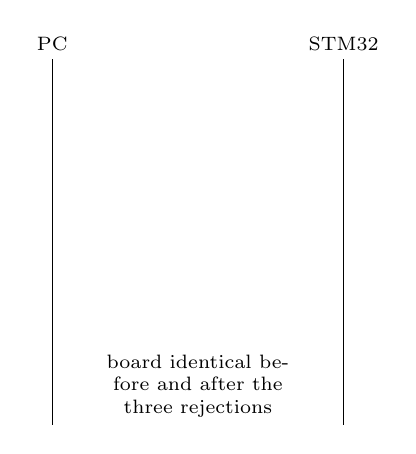
\begin{tikzpicture}[x=1cm,y=1cm]
 \node[font=\scriptsize] at (0,0.35) {PC};\node[font=\scriptsize] at (3.7,0.35) {STM32};
 \draw (0,0.15) -- (0,-4.5);\draw (3.7,0.15) -- (3.7,-4.5);
 \seqpair{-0.05}{MOVE:4:O}{NACK:OCCUPIED}
 \seqpair{-0.98}{MOVE:9}{NACK:RANGE}
 \seqpair{-1.91}{MOVE:4:O*00}{NACK:BADSUM}
 \seqpair{-2.84}{STATE}{BOARD:....X....}
 \node[font=\scriptsize,text width=3cm,align=center] at (1.85,-4.0) {board identical before and after the three rejections};
\end{tikzpicture}\\[2pt]{\footnotesize (b) rejections (board \code{....X....})}
\end{minipage}

\caption{Sequence diagrams (checksums omitted; solid = request, dashed = reply). (a)~A scripted X win. (b)~Three rejections leave the board unchanged.}
\label{fig:sequence}
\end{figure*}

\section{Specification and Design}
\label{sec:design}

\subsection{Pure logic is separated from hardware, and the board decides everything}
Table~\ref{tab:arch} divides the system. \code{game.c} and \code{server.c} contain no HAL or CMSIS calls, so the
identical files are compiled for the Cortex-M0 and for the PC test builds; only \code{uart.c}, \code{main.c}
and the button/LED code touch registers. The server owns the board, the turn, legality, win detection, the computer opponent's moves and
the reply text. The client owns only presentation (drawing, score, sound) and the timing of its own requests. It never
computes a legal move or a winner, so a buggy or hostile client can at worst be refused.

\begin{table}[t]
\centering
\caption{Modules and who owns each decision.}
\label{tab:arch}
\scriptsize
\begin{tabular}{@{}L{1.9cm}L{1.0cm}L{4.9cm}@{}}
\toprule
Module & HAL? & Responsibility \\
\midrule
\code{game.c} & no & 10-byte state, validate-then-commit, 8-line win test \\
\code{server.c} & no & byte-driven framer, parser, checksum, dispatch to \code{game.c} \\
\code{ai.c} & no & minimax opponent for O; only picks a cell, the move goes through \code{game.c} \\
\code{uart.c} & yes & USART1 RX interrupt, 128-byte ring, polled TX \\
\code{main.c} & yes & loop: drain ring, \code{server_rx}, \code{server_tick}, button, LED \\
\code{client.py} & no & protocol client, checksum check, \code{GameView} (no Tk) \\
\code{app.py} & Tk & canvas, worker thread, score, sound \\
\bottomrule
\end{tabular}
\end{table}

\subsection{The server FSM validates before it commits}
Figure~\ref{fig:fsm} shows the three states. IDLE accepts \code{CONNECT}, \code{NEW} and \code{DISCONNECT}. IN\_PROGRESS accepts
\code{MOVE}, \code{STATE} and \code{RESIGN}, and GAME\_OVER accepts \code{NEW}, \code{STATE} and \code{DISCONNECT}. The \code{MOVE}
branch runs the checks range, turn, occupancy in that order, each with its own NACK exit that returns to IN\_PROGRESS
without writing. Only a move passing all three is committed; the win or draw test then decides between IN\_PROGRESS and
GAME\_OVER. The button resets to IDLE from any state. The figure omits the framer errors, which never reach the FSM
(Table~\ref{tab:framing}).

\begin{figure*}[t]
\centering
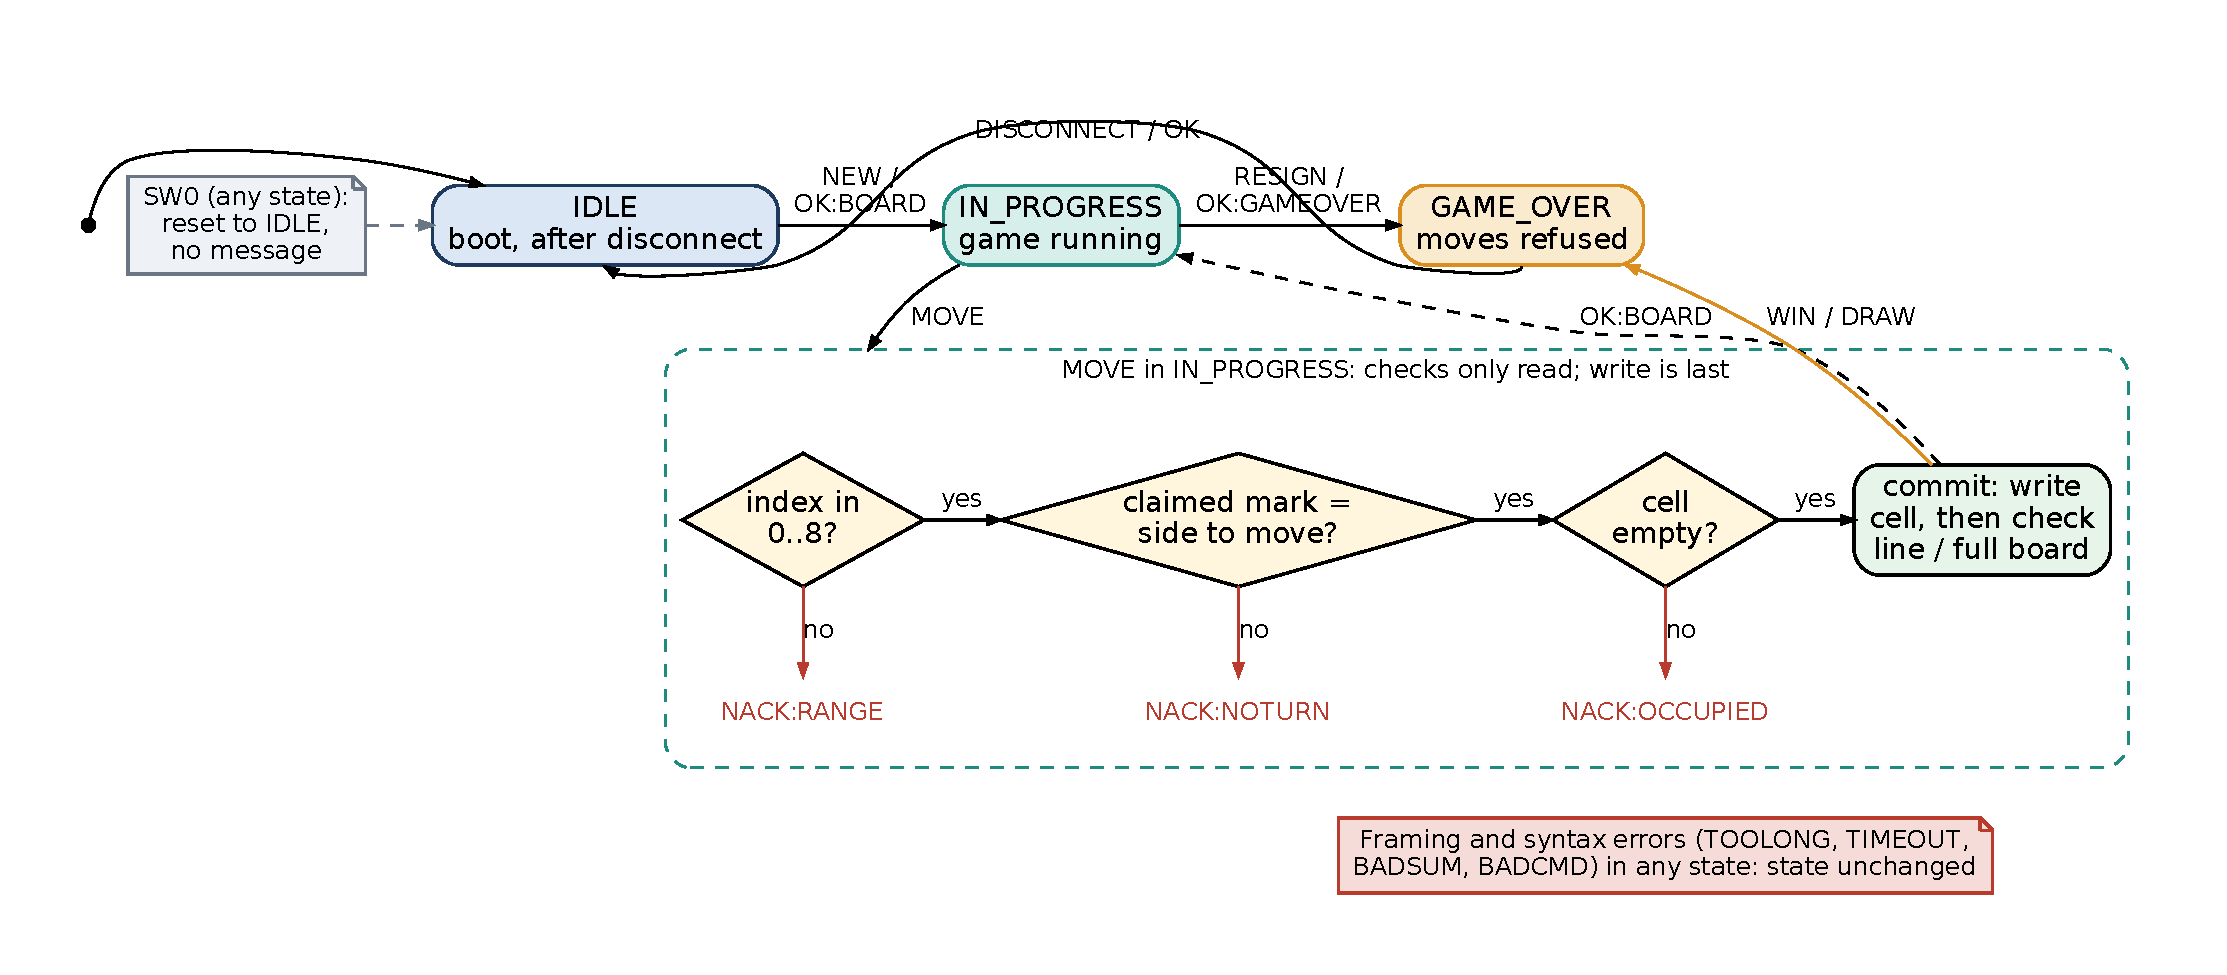
\includegraphics[width=\textwidth]{figures/fsm.pdf}
\caption{Server FSM with the \code{MOVE} validation branch. Transitions read ``command [guard] / reply''.}
\label{fig:fsm}
\end{figure*}

\subsection{The GUI never draws before the server confirms}
Figure~\ref{fig:gui} shows the client flow. A request is placed on a worker thread, so the Tk main loop never waits on the serial
port, and the main loop polls a result queue every 30~ms. On a reply the client first verifies the checksum; a missing or wrong
one counts as not received. Only a verified \code{OK:BOARD}, \code{WIN}, \code{DRAW} or \code{BOARD} reply redraws the
board, and a NACK shows its message and leaves the display as it was. A click on an occupied cell is sent anyway, so the board's \code{NACK:OCCUPIED} is what the user sees: the GUI does not decide legality. After a win, draw or resign, cells are disabled until
\code{NEW}. On a lost reply (1~s timeout) the client sends \code{STATE} once and redraws from it, because \code{STATE} is safe
to repeat; if that also fails it reports ``server not responding''. If a \code{MOVE} is answered \code{NACK:NOGAME}
mid-game, the board was reset by its button, so the client returns to the start screen.

\begin{figure*}[t]
\centering
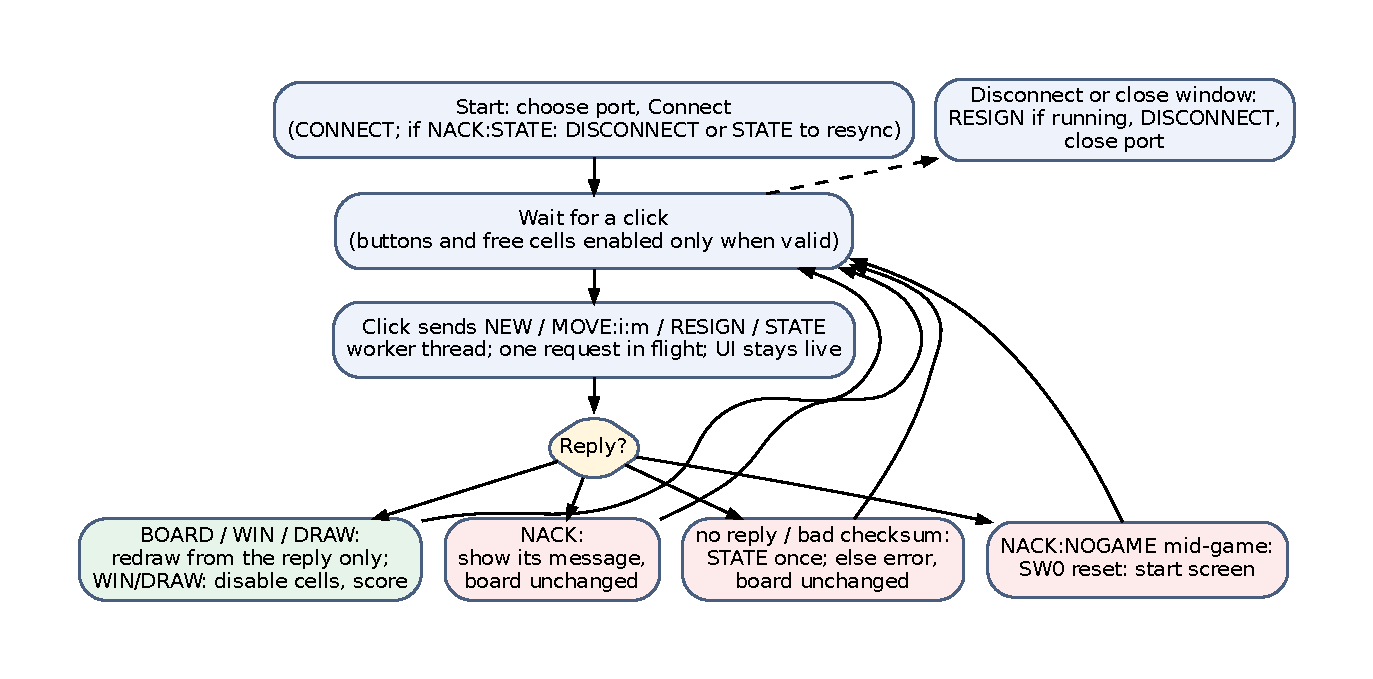
\includegraphics[width=0.78\textwidth]{figures/gui_flow.pdf}
\caption{GUI flowchart: requests run on a worker thread and the display changes only on a verified reply.}
\label{fig:gui}
\end{figure*}

\subsection{The USB cable is the UART link; SW0 and the LED are local}
Figure~\ref{fig:circuit} shows the connection. No adapter is used: the on-board ST-Link bridges USART1 to a USB virtual COM
port, with TX on PA9 and RX on PA10 (alternate function AF1, datasheet Table~14~\cite{ds8668}). SW0 on PA0 is active low with
the internal pull-up; a press resets the game to IDLE. The red LED is on PB10 and the green on PB11, each through 150~$\Omega$
(schematic~\cite{schematic}). The LED is off in IDLE, green while X is to move, red while O is to move, and both blink together
at 2~Hz (250~ms half-period in code) in GAME\_OVER.

\begin{figure}[t]
\centering
\resizebox{\linewidth}{!}{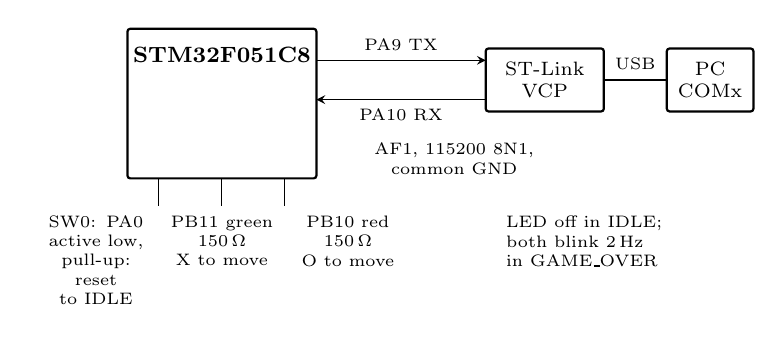
\begin{tikzpicture}[x=1cm,y=1cm,font=\scriptsize,
  box/.style={draw,thick,rounded corners=1pt,align=center,inner sep=2pt}]
 \node[box,minimum width=2.4cm,minimum height=1.9cm] (mcu) at (0,0) {};
 \node[font=\footnotesize\bfseries] at (0,0.62) {STM32F051C8};
 \node[box,minimum width=1.5cm,minimum height=0.8cm] (stl) at (4.1,0.3) {ST-Link\\VCP};
 \node[box,minimum width=1.1cm,minimum height=0.8cm] (pc) at (6.2,0.3) {PC\\COMx};
 \draw[->,>=stealth] (1.2,0.55) -- node[above,font=\fontsize{6}{7}\selectfont]{PA9 TX} (3.35,0.55);
 \draw[<-,>=stealth] (1.2,0.05) -- node[below,font=\fontsize{6}{7}\selectfont]{PA10 RX} (3.35,0.05);
 \draw[thick] (4.85,0.3) -- node[above,font=\fontsize{6}{7}\selectfont]{USB} (5.65,0.3);
 \node[font=\fontsize{6}{7}\selectfont,align=center] at (2.95,-0.7) {AF1, 115200 8N1,\\common GND};
 \foreach \x/\t in {-1.6/{SW0: PA0\\active low,\\pull-up: reset\\to IDLE}, 0/{PB11 green\\150\,$\Omega$\\X to move}, 1.6/{PB10 red\\150\,$\Omega$\\O to move}}{
   \draw (\x*0.5,-0.95) -- (\x*0.5,-1.3);
   \node[below,align=center,text width=1.5cm,font=\fontsize{6}{7}\selectfont] at (\x,-1.3) {\t};}
 \node[align=left,font=\fontsize{6}{7}\selectfont] at (4.6,-1.75) {LED off in IDLE;\\both blink 2\,Hz\\in GAME\_OVER};
\end{tikzpicture}
}
\caption{UART path to the PC and the button and LED pins.}
\label{fig:circuit}
\end{figure}

\section{Implementation}
\label{sec:impl}

\subsection{The interrupt only moves bytes; the main loop does the work}
At 115200 baud a byte arrives every 87~\textmu s, and the USART has a one-byte receive register, so a second byte overwrites the first
if the program is busy elsewhere (overrun). Listing~\ref{lst:irq} is the whole receive interrupt: it reads \code{RDR},
stores the byte in a 128-byte ring buffer and returns. The ring has a power-of-two size so the wrap is a mask, and it is written
only by the interrupt (\code{head}) and read only by the main loop (\code{tail}), so no lock is needed. If the ring is full the
byte is counted and dropped rather than waiting. The error flags (overrun, framing, noise) are cleared by writing \code{ICR}, as described in the reference manual~\cite{rm0091}, so that one error does not persist.
We trimmed the declarations.

\begin{figure}[t]
\begin{lstlisting}[float=false,language=C, caption={Receive interrupt and ring buffer (\texttt{uart.c}, trimmed).}, label=lst:irq]
void USART1_IRQHandler(void){
  uint32_t isr = USART1->ISR;
  if (isr & (USART_ISR_ORE|USART_ISR_FE|USART_ISR_NE)) {
    if (isr & USART_ISR_ORE) overruns++;
    USART1->ICR = USART_ICR_ORECF | USART_ICR_FECF
                | USART_ICR_NCF;    /* clear flags */
  }
  if (isr & USART_ISR_RXNE) {
    uint8_t b = (uint8_t)USART1->RDR;  /* clears RXNE */
    uint16_t next = (head + 1u) & (RING_SZ - 1u);
    if (next != tail) { ring[head] = b; head = next; }
    else dropped++;           /* full: drop, never wait */
  }
}
\end{lstlisting}
\end{figure}

\subsection{The framer replies at the 33rd byte and resynchronises at the next LF}
Listing~\ref{lst:framer} shows the byte-driven framer. The obvious alternative is to collect bytes until the LF and then test
the length, but a sender that never sends LF would then fill the buffer or stall the server. Here the 33rd byte produces
\code{NACK:TOOLONG} immediately and moves to a DISCARDING state that drops bytes silently until the next LF, so an oversize frame
gets one reply, not two, and the buffer cannot overflow. Each call writes at most one reply and never waits. The inactivity
timer is checked in \code{server_tick}, not with a delay, using the unsigned difference \code{now - last_ms}. This caused a bug: the
main loop first read the time and then drained the ring, so \code{last_ms} could be newer than \code{now} and the unsigned subtraction
wrapped to about $4\times10^9$, producing a false \code{NACK:TIMEOUT}. We found it by reading the code before the first flash and fixed
it by reading the clock \emph{after} the drain, as the comment in \code{main.c} records.

\begin{figure}[t]
\begin{lstlisting}[float=false,language=C, caption={Framer (\texttt{server.c}, trimmed). At most one reply per call.}, label=lst:framer]
size_t server_rx(server_t *s, uint8_t byte,
   uint32_t now_ms, char *out, size_t cap){
  size_t n = 0;  s->last_ms = now_ms;
  switch (s->rx) {
  case RX_IDLE: case RX_RECEIVING:
    if (byte == LF) {          /* len 0: empty frame */
      n = handle_frame(s, s->buf, s->len, out, cap);
      server_reset_framer(s);
    } else if (s->len >= SERVER_MAX_FRAME) { /*33rd*/
      n = make_reply("NACK:TOOLONG", out, cap);
      s->len = 0;  s->rx = RX_DISCARDING;
    } else { s->buf[s->len++] = (char)byte;
             s->rx = RX_RECEIVING; }
    break;
  case RX_DISCARDING:
    if (byte == LF) server_reset_framer(s);
    break;
  }
  return n;
}
\end{lstlisting}
\end{figure}

\subsection{The GUI does serial I/O on a worker thread and draws on a timer}
A \code{MOVE} can take up to the 1~s reply timeout, and a Tk window that waits for it stops redrawing and looks frozen. Listing~\ref{lst:gui}
runs each exchange on a daemon thread and passes the result back through a queue; only the Tk thread touches widgets. \code{poll}
drains the queue every 30~ms using \code{root.after}, which is Tk's thread-safe way to schedule work on its own loop. The three
exception paths separate a protocol error (\code{ReplyError}, shown as a message), and anything else such as a missing or unplugged
port (``fatal'', disconnect), so an unexpected failure can never leave the \code{busy} flag set and lock the board. The
\code{exchange} method sends \code{STATE} once after a lost reply, as described in Sec.~\ref{sec:design}.

\begin{figure}[t]
\begin{lstlisting}[float=false,language=Python, caption={GUI worker thread and queue polling (\texttt{app.py}, trimmed).}, label=lst:gui]
def run_in_thread(self, work):
    self.busy = True; self.refresh()
    def target():
        try:    self.results.put(("ok", work()))
        except ReplyError as exc:
            self.results.put(("err", str(exc)))
        except Exception as exc:  # port gone
            self.results.put(("fatal", str(exc)))
    threading.Thread(target=target, daemon=True).start()

def poll(self):
    try:
        while True:
            kind, payload = self.results.get_nowait()
            self.finish(kind, payload)
    except queue.Empty: pass
    self.root.after(30, self.poll)
\end{lstlisting}
\end{figure}

\section{Game Logic and Server Authority}
\label{sec:authority}

\subsection{All state is 10 bytes owned by the STM32}
The whole game is one \code{game_t}: nine cells and a state byte, 10 bytes with no padding. The client never holds it; it receives
only checksummed text replies. The side to move is computed from the board (X when the counts are equal), so there is no separate turn variable that could
disagree with the board, and a client cannot make it disagree.

\subsection{A rejection cannot change state because every check precedes the first write}
Listing~\ref{lst:move} is \code{game_move}. Every error \code{return} appears before the line \code{g->board[index] = side}, and the
checks only read \code{*g}. The proof is by inspection: a path that returns an error has executed no write, so there is nothing to undo.
The other commands share the shape of one condition followed by at most one state change. The order of the checks (state, range, turn,
occupancy) is the order in Table~\ref{tab:errors}, and it is the same order the protocol promises, so the choice of NACK is deterministic.

\begin{figure}[t]
\begin{lstlisting}[float=false,language=C, caption={Validate-then-commit (\texttt{game.c}, comments trimmed).}, label=lst:move]
if (g->state != GAME_IN_PROGRESS) return GAME_ERR_NOGAME;
if (index < 0 || index >= GAME_CELLS)
                                  return GAME_ERR_RANGE;
const char side = game_side_to_move(g);
if (mark != 0 && mark != side)    return GAME_ERR_NOTURN;
if (g->board[index] != '.')       return GAME_ERR_OCCUPIED;
/* ---- commit: first write to *g ---- */
g->board[index] = side;
const game_result_t r = game_evaluate(g->board);
if (r != GAME_RESULT_NONE) g->state = GAME_OVER;
\end{lstlisting}
\end{figure}

\subsection{The AI opponent cannot bypass the rules}
In a \code{NEW:AI} game the server picks O's cell with \code{ai_pick}, which only reads a copy of the board, and then makes the move through the same \code{game_move} shown in Listing~\ref{lst:move}. It therefore cannot play an occupied or out-of-range cell. The AI flag is kept in the server structure, not in \code{game_t}, so the 10-byte game and the exhaustive core tests are unchanged. The search is minimax with alpha-beta pruning, so O never loses. We checked this on the PC by letting X try every possible sequence of moves: 681 games, 0 X wins (498 O wins, 183 draws), and 936 AI moves, none illegal (\tn{test_ai.c}, PC). A rejected \code{MOVE} does not trigger an AI move (\tn{test_rejected_moves_do_not_wake_the_ai}).

\subsection{Win and draw are decided by the server after each commit}
After a commit, \code{game_evaluate} tests the eight lines (three rows, three columns, two diagonals) before testing for a full board, so a move
that fills the last cell and completes a line is a win, not a draw. The server then ends the game and replies \code{WIN} or \code{DRAW}.
Table~\ref{tab:logic} lists the checks that back the argument. They run on the PC (game core alone), except the last row, which is the board suite.

\begin{table}[t]
\centering
\caption{Evidence for the authority argument (PC unless stated).}
\label{tab:logic}
\scriptsize
\begin{tabular}{@{}L{3.9cm}L{3.9cm}@{}}
\toprule
Check & Result \\
\midrule
Every error compared byte-for-byte (\code{memcmp} of the 10 bytes) & 0 failures in 50{,}546{,}417 checks \\
All positions reachable by legal play, each tried with every index and claim & 549{,}946 positions; 6{,}859{,}116 illegal attempts, all left the game identical \\
Random calls (fixed seed): six commands, indices $-3$..12 & 2{,}000{,}000 calls, invariants held; 22{,}948 wins, 3{,}003 draws \\
Independent Python brute force vs.\ C rules & 255{,}168 games: 131{,}184 X, 77{,}904 O, 46{,}080 draws; C reproduces them \\
All 8 lines, both players, over the serial link & \tn{test_each_line_wins}, 16 cases; passes on the board \\
All 936 AI moves, X plays every sequence & 681 games: 0 X wins, 0 illegal AI moves \\
\bottomrule
\end{tabular}
\end{table}

The exhaustive run covers the game core only, not framing, and it ran on a PC. It uses one fixed random seed, so it is repeatable
rather than broad. The link-level claim rests on the same invariants being tested through the serial port on the board
(Sec.~\ref{sec:valid}). Hostile clients are bounded the same way: a client that lies about the turn gets \code{NACK:NOTURN}, one that
resends a move gets \code{NACK:OCCUPIED} or \code{NACK:NOGAME}, and none of these changes the 10 bytes.

\section{Protocol Robustness and Integrity}
\label{sec:robust}

Every malformed input is answered by a specific NACK and followed by recovery: the framer returns to its idle state at the next LF, and the
game state is never touched. Table~\ref{tab:threats} maps each kind of bad input to its mechanism and test. All tests named ran on the board
(113 of 113 passed, Sec.~\ref{sec:valid}), except where noted.

\begin{table}[t]
\centering
\caption{Bad input, the server's handling, and the test that checks it.}
\label{tab:threats}
\scriptsize
\begin{tabular}{@{}L{1.5cm}L{3.0cm}L{3.4cm}@{}}
\toprule
Bad input & Handling and response & Test \\
\midrule
Partial frame & 500 ms inactivity timer; \code{NACK:TIMEOUT}; remainder is a new frame & \tn{test_partial_frame_times_out}, \tn{test_inactivity_timer_restarts_on_each_byte} \\
Oversize (33+ bytes) & \code{NACK:TOOLONG} at byte 33, skip to LF & \tn{test_32_byte_frame_accepted_33_rejected}, \tn{test_oversize_frames_get_exactly_one_nack} \\
Garbage bytes & \code{NACK:BADCMD} per LF; next valid frame answered & \tn{test_random_garbage_never_breaks_the_server}, \tn{test_garbage_does_not_change_game} \\
Unknown or wrong-case command & \code{NACK:BADCMD} & \tn{test_bad_command_variants} \\
Corrupted bytes & XOR check; \code{NACK:BADSUM}; never executed & \tn{test_bad_checksum_never_executes_command} \\
Pipelined burst of 32+ frames & Replies lost (see text); not handled & \tn{measure\_board.py} M4 \\
UART errors (overrun, framing) & ISR clears flags, counts; no reply possible & not tested on the board (counters cannot be read without writing to the game UART) \\
\bottomrule
\end{tabular}
\end{table}

\subsection{A 500 ms inactivity timer abandons stalled frames}
A full 32-byte frame takes about 2.8~ms at 115200 baud, so 500~ms fires only when a sender has really stalled, while a person typing in a terminal
(whose bytes arrive in bursts of a line) is not cut off. The timer restarts on every byte and runs only while a frame is in progress, so an idle line costs nothing.
The timeout is 500~ms in the code and the protocol. The measurements M1--M5 in this section were taken on the final firmware, with the AI included. On the board the observed timeout was 500.93--502.74~ms over 20 samples (median 501.73~ms), measured from the last byte sent to the arrival of \code{NACK:TIMEOUT} (\code{board_measurements.txt}, M2), so it is within 2.8~ms of the 500~ms specification.

\subsection{Oversize and garbage input resynchronise at the next LF}
Oversize input gets one \code{NACK:TOOLONG} at the 33rd byte and is then skipped silently to the next LF
(\tn{test_discarding_times_out_silently} covers the case with no LF at all). Random binary data produces one reply per LF, which the tests count, and a
valid frame afterwards is answered correctly. In 100 random garbage frames, each followed by \code{CONNECT}, 0 recoveries failed (M5, board).

\textbf{Limit found: back-to-back bursts.} M4 sent $N$ identical \code{STATE} frames (9 bytes each) in a single write, 30 times per $N$. For $N\le16$ (144 bytes) all replies were correct (0 of 480 missing or wrong at $N=16$). At $N=32$ (288 bytes) 145 of 960 replies were missing or wrong, and at $N=64$ (576 bytes) 962 of 1920. So the one-reply-per-frame guarantee (R1) holds on the board only while the client does not pipeline more than 16 frames; our client sends one request and waits, which M3 shows is reliable. The cause is probably the 128-byte receive ring filling while the polled transmit of each reply (about 1.2~ms for 14 bytes) holds up the main loop, since the input arrives faster than replies can be sent. We did not confirm this, because the drop counter cannot be read without writing to the game UART. A larger ring or an interrupt-driven transmit would be the fix; we did not make it.

\subsection{Integrity: XOR catches every single-bit error but not swapped bytes}
We computed the checksum's limits on the PC (\code{checksum_analysis.txt}): 0 of 2{,}512 single-bit errors are missed, 11.40\% of two-bit errors are missed,
100\% of adjacent byte swaps are missed, and 0.417\% of random bodies pass by chance. XOR is therefore adequate against a single corrupted byte on a short USB cable, and it is not a defence
against an adversary. The GUI treats a reply with a bad checksum as not received.

\subsection{The server cannot block forever}
Every loop is bounded. The main loop drains the ring buffer, which holds at most 128 bytes, and never waits for input. The framer holds 32 bytes and handles one byte per call. A reply is at most 25 bytes, so the polled transmit
takes about 2.2~ms. Each byte waits for the USART's transmit-empty flag, which the hardware sets within one byte time (87~\textmu s); there is no software time-out on that wait, so a faulty USART would stall the loop, and we have not tested that case. The input timeout is a comparison of two timestamps, not a delay. No watchdog is used. Measured on the board: 2000 consecutive request/reply exchanges gave 0 wrong or missing replies at 293.6 requests/s (M3), and the request-to-reply latency for \code{STATE} over 300 samples was min 2.62, median 3.02, 95th percentile 3.83 and max 4.42~ms (M1). This latency is seen from the PC and includes the ST-Link USB path, so it is not the firmware's processing time alone. M1 uses \code{STATE}, so it does not include an AI move, whose time on the board we did not measure.

\section{Validation}
\label{sec:valid}

\subsection{One pytest suite runs on three targets}
The harness uses pytest~\cite{pytest} and pySerial~\cite{pyserial}. It opens the port given by \code{--port}: a COM port for the board, or
\code{socket://127.0.0.1:PORT} for a Python mock server or for the real \code{server.c} and \code{game.c} compiled for the PC and exposed on a TCP socket.
The tests, the GUI and the board therefore share one code path. Every test starts with a known state, and the suite needs no human
action. Run with \code{python -m pytest tests --port COM9}. Results labelled \emph{PC} below were not run on the board.

\subsection{All 113 tests pass on the board; the suite detects 15 of 15 injected faults}
Table~\ref{tab:required} maps each required case of the brief to a named test. Together with the state-table and robustness tests, the board
run on the final firmware is \textbf{125 passed in 55.13~s}: 113 tests on the board (29 required and win-line tests, 18 state-table tests, 53 robustness tests and 13 AI tests) plus 12 GUI-logic tests that run on the PC against the mock (\code{ai_board_pytest.txt}). Before the AI was added the 100 original tests also passed on the board (91.96~s, \code{stage7_board_pytest.txt}). The
same tests pass on the mock and on the PC build of the real C logic (PC). The AI row covers the optional \code{NEW:AI} opponent: 13 further tests in \tn{test_ai.py} pass on the mock, on the PC build of the real C logic (113 of 113 with the original 100) and on the board (above).

A passing suite proves little unless it can fail. We injected 15 faults into the mock (for example a NACK:NOTURN that flips the turn anyway, an occupied cell that is overwritten, index 9 accepted, a stalled frame that never times out); the suite caught all 15 (PC mock, \code{stage3_mutation_check.txt}). The first run caught 14: a
fault in the 2-4-6 diagonal went unnoticed because we tested too few lines, so we added a test for all 8 lines for both players (16 cases).

\begin{table}[t]
\centering
\caption{The brief's required tests and their results on the board.}
\label{tab:required}
\scriptsize
\begin{tabular}{@{}L{3.5cm}L{3.5cm}c@{}}
\toprule
Requirement (brief, p.~4) & Test name & Result \\
\midrule
\code{CONNECT} gives \code{OK}; \code{NEW} gives empty board & \tn{test_connect_in_idle}, \tn{test_new_game_returns_empty_board} & pass \\
Legal move changes the board as expected & \tn{test_valid_move_updates_board} & pass \\
Occupied cell: \code{NACK:OCCUPIED}, board unchanged & \tn{test_occupied} & pass \\
Out of range: \code{NACK:RANGE} & \tn{test_range} & pass \\
Move after game over: \code{NACK:NOGAME} & \tn{test_x_wins_then_no_more_moves} & pass \\
Scripted win and draw & \tn{test_x_wins_...}, \tn{test_o_wins}, \tn{test_draw}, \tn{test_each_line_wins} & pass \\
AI never illegal (if implemented) & \tn{test_ai_never_loses_and_never_cheats_against_random_x}, exhaustive \tn{test_ai.c} (PC) & pass \\
\bottomrule
\end{tabular}
\end{table}

\subsection{Screenshot: the GUI shows the board's refusal and the board is unchanged}
Figure~\ref{fig:screenshot} is a screenshot of the GUI connected to the \emph{real board} on COM9 in a two-player game. The log on the right lists each frame (TX sent, RX checksum-verified reply): a move onto an occupied cell was sent and the board answered \code{NACK:OCCUPIED}, the status line shows ``That cell is already taken.'', and the board still shows X at cell 0 and O at cell 4. The GUI sends such clicks so that the refusal comes from the server, not from the client. The picture is cropped to the board and the log (the log is enlarged); no content was changed.

\begin{figure}[t]
\centering
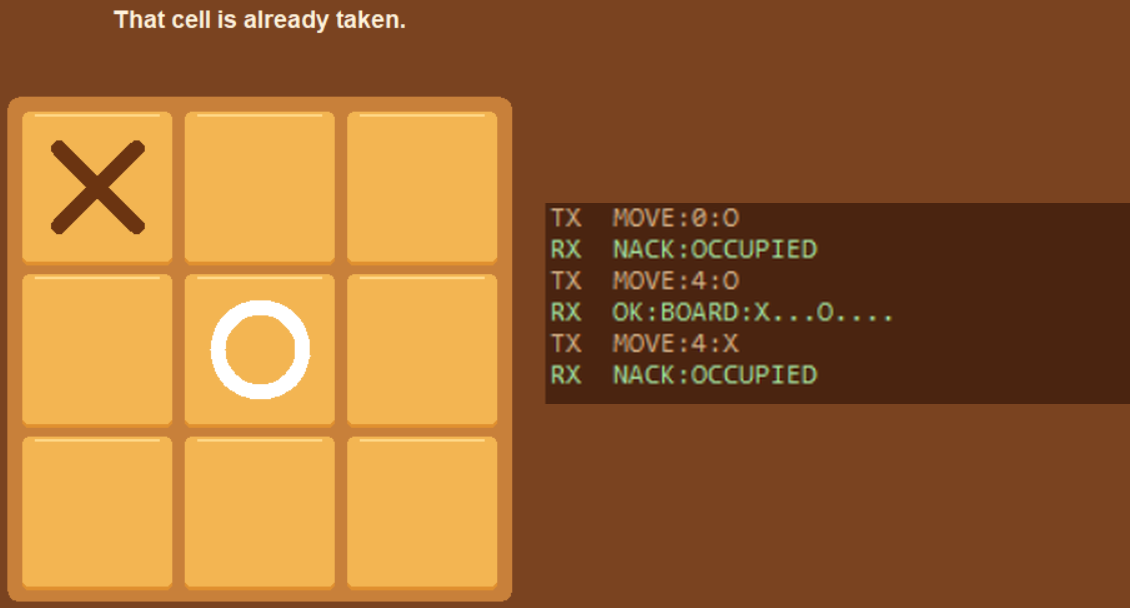
\includegraphics[width=\linewidth]{figures/gui_board_rejected.png}
\caption{GUI connected to the board (COM9): \code{NACK:OCCUPIED} twice in the log, board unchanged.}
\label{fig:screenshot}
\end{figure}

\subsection{What testing revealed}
\begin{itemize}\setlength\itemsep{0pt}
\item \emph{Timestamp underflow} in the main loop (Sec.~\ref{sec:impl}): found by code review before the first flash.
\item \emph{Diagonal gap} in the tests: found by the injected-fault run (above).
\item \emph{Fresh-clone build failure}: the Makefile's \code{mkdir build/bringup} failed when \code{build/} did not exist; we changed it to \code{mkdir -p}.
\item \emph{Read quantisation} in the test link: read latency was quantised to the 50~ms port timeout; we read \code{in_waiting} bytes instead.
\item \emph{Silent GUI sound}: \code{winsound} with \code{SND_MEMORY|SND_ASYNC} raised an error that our code swallowed; we now play from temporary WAV files. The sound plays on our PC and can be heard in the demonstration video (Sec.~\ref{sec:video}).
\item \emph{Missing ST-Link driver} on the Windows PC made the board invisible to the flash tool; installing the driver from the IDE's drivers folder fixed it.
\end{itemize}
Not tested: unplugging the cable mid-game (the GUI's lost-reply path is exercised on the mock only), UART overrun counts on the board, and the
button debounce time (30~ms is the configured value, not a measurement). The LED behaviour was observed, not measured: green when X is to move, red when O is to move, both blinking in GAME\_OVER and off after SW0 is pressed, as shown in the demonstration video; we did not time the blink, so ``2~Hz'' is the configured value only.

\section{Conclusion}
\label{sec:conclusion}

We built a Tic-Tac-Toe server on an STM32F051 that holds a 10-byte game, refuses every illegal request without changing it,
and answers each frame with exactly one reply when the client waits for replies. The evidence is a 113-test suite that passes on the board (125 of 125 passed in 55.13~s with the 12 GUI-logic tests) and also on the mock and on the C logic compiled for the PC, and a
fault-injection check that catches 15 of 15 faults. The firmware image is 6{,}420 bytes of code in 64~KB flash, with 1{,}772 bytes of static RAM in 8~KB.

Limits are as follows. XOR misses all adjacent byte swaps and 11.40\% of two-bit errors, so it guards against line noise, not an attacker. Pipelining is limited: when 32 frames were sent in one write, 145 of 960 replies were lost on the board (16 frames were reliable), so the guarantee of one reply per frame holds for request-and-wait clients, which is how our GUI and tests behave. The protocol supports one client and
no hidden information. We did not implement the move clock or undo. The AI move is computed in the main loop before the reply is sent; it takes about 142~\textmu s on a PC and we have not measured it on the board. The overrun counters exist but cannot be read without writing to the game UART, so
we do not claim a number for UART errors on the board. With more time we would add a hardware-timer move clock and a larger receive buffer.

\section{Video}
\label{sec:video}

The demonstration video is at \url{https://uctcloud-my.sharepoint.com/:v:/g/personal/mkmosw001_myuct_ac_za/IQBZcJdG0mWPTJIXVgzibqDiAV5_YdHbaOCg49HO0I2NqBA?e=v53mvg&nav=eyJyZWZlcnJhbEluZm8iOnsicmVmZXJyYWxBcHAiOiJTdHJlYW1XZWJBcHAiLCJyZWZlcnJhbFZpZXciOiJTaGFyZURpYWxvZy1MaW5rIiwicmVmZXJyYWxBcHBQbGF0Zm9ybSI6IldlYiIsInJlZmVycmFsTW9kZSI6InZpZXcifX0\%3D}. It shows the game running on the STM32 board with the GUI: connecting, legal moves, a rejected move, a win, a new game, the board's LED and SW0 button, and a game against the computer, with sound, and disconnecting.

\section{Code}
\label{sec:code}

The source code is at \url{https://github.com/OswikaMukoma/Tic-Tac-Toe}. The repository holds the firmware (Makefile, imports into STM32CubeIDE), the Tkinter GUI, the pytest harness with the mock and PC servers, the protocol specification and the evidence files. Setup, build, flash, run and test instructions are in its \code{README.md}.


\bibliographystyle{IEEEtran}
\bibliography{refs}

\end{document}
